\section{The CRB at the TCP centre}\label{sec:crb}

\subsection{Point value and limit}
Write $x\equiv L^2\ln2/\fwhm^2$ and $g\equiv1-x$ ($x<1$, i.e.\ the peripheral zeros lie inside
the ring maximum). At $\rr=\mathbf0$ the central exposure has $p_3=0$ and $\nabla p_3=0$, so its
term in Eq.~\eqref{eq:fisher} is $0/0$. Dropping it gives the \emph{point value}, Balzarotti's
Eq.~S27 \cite{Balzarotti2017}:
\begin{equation}
\sigma_{\mathrm{pt}}=\frac{L}{2\sqrt{2N}}\,g^{-1}.
\label{eq:s27}
\end{equation}
For $\rr\neq\mathbf0$, however, $p_3\propto r^2$ and $\nabla p_3\propto\rr$, so the central term
tends to a finite matrix of fixed norm along $\rhat\rhat^{T}$. The limit $r\to0$ of the bound is
(App.~\ref{app:derivation})\src{deriv_limit}
\begin{equation}
\sigma_{\lim}^2=\frac{L^2}{8Ng^2}\,\frac{3g^2+e^{x}}{3g^2+2e^{x}},\qquad
\rho\equiv\frac{\sigma_{\lim}}{\sigma_{\mathrm{pt}}}=\sqrt{\frac{3g^2+e^{x}}{3g^2+2e^{x}}}.
\label{eq:limit}
\end{equation}
It does not depend on the direction of approach, so it is a well-defined, direction-independent
``centre CRB'' (the limiting error ellipse itself is anisotropic, see below). For $L=50$\,nm, $N=100$ and $\fwhm=\pnum{fwhm_nm}\src{fwhm_nm}$\,nm the numerical limit
of Eq.~\eqref{eq:crb} (12 directions at $|\rr|=10^{-3}$\,nm) is
\pnum{crb_center_lg_L50_N100_nm}\src{crb_center_lg_L50_N100_nm}\,nm and the closed form gives
\pnum{crb_center_lg_L50_N100_closed_nm}\src{crb_center_lg_L50_N100_closed_nm}\,nm, while the
point value is \pnum{crb_center_point_S27_L50_N100_nm}\src{crb_center_point_S27_L50_N100_nm}\,nm.
The closed forms agree with an independent numerical Fisher computation in all tested cases\src{check_closed_forms}. We use the limit because it describes an emitter at any small but
non-zero distance from the centre; the point value describes a set of measure zero.

For a quadratic zero ($x\to0$) the ratio is exactly $\rho=2/\sqrt5$, i.e.\
$\sigma^2_{\lim}=L^2/(10N)$ against $\sigma^2_{\mathrm{pt}}=L^2/(8N)$:
$\rho=\pnum{limit_to_point_ratio_quadratic}\src{limit_to_point_ratio_quadratic}$ (numerically,
with $\fwhm=10^9$\,nm, \pnum{limit_to_point_ratio_quadratic_numeric}\src{limit_to_point_ratio_quadratic_numeric}).
With finite $\fwhm$ the ratio is not conserved: at $\fwhm=\pnum{fwhm_nm}\src{fwhm_nm}$\,nm it is
\pnum{limit_to_point_ratio_L5}\src{limit_to_point_ratio_L5},
\pnum{limit_to_point_ratio_L50}\src{limit_to_point_ratio_L50},
\pnum{limit_to_point_ratio_L100}\src{limit_to_point_ratio_L100} and
\pnum{limit_to_point_ratio_L150}\src{limit_to_point_ratio_L150} for $L=5$, $50$, $100$ and
$150$\,nm [Fig.~\ref{fig:crbmaps}(f)], because the peripheral term scales as $g^2$ while the
central one scales as $e^{x}$.

\emph{Origin of the discontinuity.} The central term tends to $(\beta/N)\,\rhat\rhat^{T}$
($\alpha$ and $\beta$ are defined in Eq.~\eqref{eq:alphabeta}), which has a limit in norm but not as a matrix; equivalently $\sqrt{p_3}\propto|\rr|$ is a cone, so the
differentiability of $\sqrt{p}$ required by the Cram\'er--Rao theorem fails exactly at $r=0$\src{deriv_discontinuity}. The central exposure contributes only radial information, of the same
size at any distance (a quadratic zero is scale invariant), and a zero count is informative.
The limiting error ellipse is therefore anisotropic: $\sigma_\parallel=(\alpha+\beta)^{-1/2}$
along $\rhat$ and $\sigma_\perp=\sigma_{\mathrm{pt}}$ across it (App.~\ref{app:derivation}); for
$L=50$\,nm, $N=100$ these are
\pnum{crb_limit_axis_par_L50_N100_nm}\src{crb_limit_axis_par_L50_N100_nm}\,nm and
\pnum{crb_limit_axis_perp_L50_N100_nm}\src{crb_limit_axis_perp_L50_N100_nm}\,nm; for a quadratic
zero ($L=100$\,nm, $N=100$) \pnum{crb_limit_axis_par_L100_N100_quadratic_nm}\src{crb_limit_axis_par_L100_N100_quadratic_nm}\,nm
and \pnum{crb_limit_axis_perp_L100_N100_quadratic_nm}\src{crb_limit_axis_perp_L100_N100_quadratic_nm}\,nm,
with ratio $\sqrt{3/5}=\pnum{crb_limit_axis_ratio_quadratic}\src{crb_limit_axis_ratio_quadratic}$.

\subsection{Background: continuity and non-commuting limits}
With a finite SBR, $p_3\ge(1-s)/K>0$ with $s=\sbr/(\sbr+1)$, the central term vanishes as $r^2$
and the bound is continuous; the point value equals the limit and Balzarotti's Eq.~S31,
\begin{equation}
\crb(\mathbf0)=\frac{L}{2\sqrt{2N}}\,g^{-1}\sqrt{\Big(1+\frac{1}{\sbr}\Big)\Big(1+\frac{3}{4\,\sbr}\Big)}.
\label{eq:s31}
\end{equation}
For $\sbr=10$, $L=50$\,nm and $N=100$, Eq.~\eqref{eq:s31} gives
\pnum{crb_center_sbr10_L50_N100_nm}\src{crb_center_sbr10_L50_N100_nm}\,nm and the numerical
limit \pnum{crb_center_sbr10_limit_L50_N100_nm}\src{crb_center_sbr10_limit_L50_N100_nm}\,nm
[Fig.~\ref{fig:crbmaps}(e)]. The two limits do not commute\src{deriv_noncommuting}:
$\lim_{\sbr\to\infty}\lim_{r\to0}\crb=\sigma_{\mathrm{pt}}$ whereas
$\lim_{r\to0}\lim_{\sbr\to\infty}\crb=\sigma_{\lim}$; the central term switches on over a radius
$r_c\propto\sbr^{-1/2}$ that shrinks to a point [Fig.~\ref{fig:scaling}(c)]. To leading order
$r_c\simeq(\sqrt3L/4)\,e^{-x/2}/\sqrt{\sbr}$ (App.~\ref{app:derivation}): at realistic SBR it is
not small compared with $L$ (where the leading-order estimate is only indicative), and
Eq.~\eqref{eq:s31} is then the relevant centre value.

\subsection{Maps and scaling}
Figure~\ref{fig:crbmaps}(a--d) shows the CRB over the field of view for $L=50$ and $100$\,nm,
with and without background. The precision is best near the centre and degrades outside the
circle of zeros.

\emph{Scaling with $L$ and $N$.} For $L\ll\fwhm$ the centre CRB is linear in $L$: the log--log
slope over $L=5$--$40$\,nm is \pnum{crb_exponent_L}\src{crb_exponent_L}
[Fig.~\ref{fig:scaling}(a)]. The exponent is range dependent: over larger $L$ the factor
$g^{-1}$ steepens the curve, and with a perfect zero the bound diverges at the ring diameter
$L=\fwhm/\sqrt{\ln2}=\pnum{eps0_crb_divergence_L_nm}\src{eps0_crb_divergence_L_nm}$\,nm and
decreases beyond. The dependence on $N$ is exactly $N^{-1/2}$ (slope
$\pnum{crb_exponent_N}\src{crb_exponent_N}$ over $N=10^2$--$10^4$) for the limit, Eq.~\eqref{eq:s27} and Eq.~\eqref{eq:s31}
[Fig.~\ref{fig:scaling}(b)].

\emph{Photon cost of background.} The photons needed for a $5$\,nm centre CRB at $L=50$\,nm
(point value, Eqs.~\eqref{eq:s27} and~\eqref{eq:s31}) are
\pnum{photons_for_5nm_L50_sbrinf}\src{photons_for_5nm_L50_sbrinf},
\pnum{photons_for_5nm_L50_sbr50}\src{photons_for_5nm_L50_sbr50},
\pnum{photons_for_5nm_L50_sbr20}\src{photons_for_5nm_L50_sbr20},
\pnum{photons_for_5nm_L50_sbr10}\src{photons_for_5nm_L50_sbr10} and
\pnum{photons_for_5nm_L50_sbr5}\src{photons_for_5nm_L50_sbr5} for $\sbr=\infty$, $50$, $20$,
$10$ and $5$; with the background-free limit it would be
\pnum{photons_for_5nm_L50_limit_nobg}\src{photons_for_5nm_L50_limit_nobg}.

\emph{Comparison with published values and variants.} With $N=500$ and $\sbr=5$,
Eq.~\eqref{eq:s31} gives \pnum{crb_center_sbr5_N500_fwhm360_L50_nm}\src{crb_center_sbr5_N500_fwhm360_L50_nm},
\pnum{crb_center_sbr5_N500_fwhm360_L100_nm}\src{crb_center_sbr5_N500_fwhm360_L100_nm} and
\pnum{crb_center_sbr5_N500_fwhm360_L150_nm}\src{crb_center_sbr5_N500_fwhm360_L150_nm}\,nm for
$L=50$, $100$, $150$\,nm when $\fwhm=\pnum{fwhm_masullo_nm}\src{fwhm_masullo_nm}$\,nm. These
match, up to rounding in the last digit at $L=150$\,nm, the MINFLUX centre-precision column of
Supplementary Table~1 of Masullo \textit{et al.} \cite{Masullo2022}\src{lit_masullo_table};
that table legend states no SBR or $N$ for this column, so $\sbr=5$, $N=500$ and this $\fwhm$
are our inference from the other columns. By contrast, with $\fwhm=\pnum{fwhm_nm}\src{fwhm_nm}$\,nm the same
formula gives \pnum{crb_center_sbr5_N500_fwhm300_L50_nm}\src{crb_center_sbr5_N500_fwhm300_L50_nm},
\pnum{crb_center_sbr5_N500_fwhm300_L100_nm}\src{crb_center_sbr5_N500_fwhm300_L100_nm} and
\pnum{crb_center_sbr5_N500_fwhm300_L150_nm}\src{crb_center_sbr5_N500_fwhm300_L150_nm}\,nm. The
one-dimensional two-exposure bound $L/(4\sqrt N)$ (Balzarotti Eq.~S22c) is
\pnum{crb_1d_quadratic_L50_N100_nm}\src{crb_1d_quadratic_L50_N100_nm}\,nm for $L=50$\,nm,
$N=100$. With a multiphoton exponent $c$ ($\lambda_i\propto I_i^c$
\cite{MasulloStefani2022}) the point value is $\sigma_{\mathrm{pt}}/c$\src{deriv_multiphoton}: \pnum{crb_center_multiphoton_c1_L100_N100_quadratic_nm}\src{crb_center_multiphoton_c1_L100_N100_quadratic_nm},
\pnum{crb_center_multiphoton_c2_L100_N100_quadratic_nm}\src{crb_center_multiphoton_c2_L100_N100_quadratic_nm}
and \pnum{crb_center_multiphoton_c3_L100_N100_quadratic_nm}\src{crb_center_multiphoton_c3_L100_N100_quadratic_nm}\,nm
for $c=1$, $2$, $3$ ($L=100$\,nm, $N=100$, quadratic zero); for $c>1$ the central term vanishes
at the origin and there is no discontinuity.

\begin{figure*}[t]
\centering
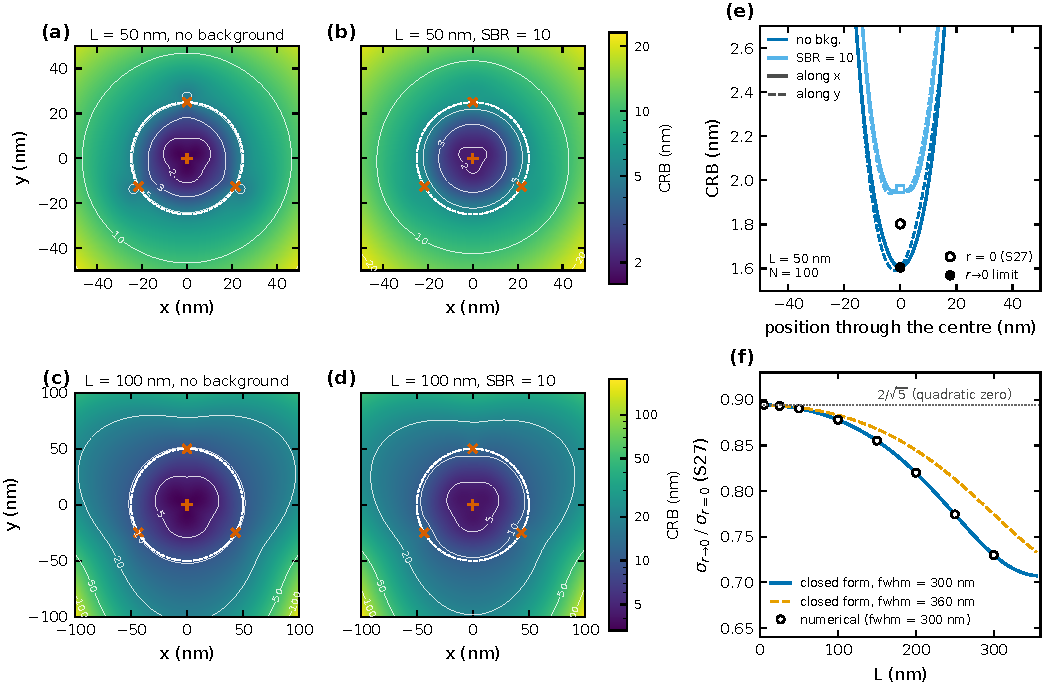
\includegraphics[width=\textwidth]{figures/fig3_crb_maps.pdf}
\caption{CRB maps and the discontinuity at the TCP centre ($\fwhm=\pnum{fwhm_nm}\src{fwhm_nm}$\,nm,
$N=100$). (a--d)~CRB over the field of view $|x|,|y|\le L$ for $L=50$ and $100$\,nm, without
background and with $\sbr=10$ (logarithmic colour scale, contours in nm; pixels on a perfect
zero take the $r\to0$ limit). (e)~Cuts through the centre along $x$ and $y$ for $L=50$\,nm:
without background the $r\to0$ limit
(\pnum{crb_center_lg_L50_N100_nm}\src{crb_center_lg_L50_N100_nm}\,nm, filled circle) lies below
the point value of Eq.~\eqref{eq:s27}
(\pnum{crb_center_point_S27_L50_N100_nm}\src{crb_center_point_S27_L50_N100_nm}\,nm, open
circle), which excludes the central exposure with $p=0$; with $\sbr=10$ the CRB is continuous
(Eq.~\eqref{eq:s31}, \pnum{crb_center_sbr10_L50_N100_nm}\src{crb_center_sbr10_L50_N100_nm}\,nm).
(f)~Ratio of the limit to the point value versus $L$, closed form (lines) and numerical Fisher
computation (circles), with the closed form for
$\fwhm=\pnum{fwhm_masullo_nm}\src{fwhm_masullo_nm}$\,nm dashed; it tends to $2/\sqrt5$ only for a quadratic zero ($L\ll\fwhm$).}
\label{fig:crbmaps}
\end{figure*}

\begin{figure*}[t]
\centering
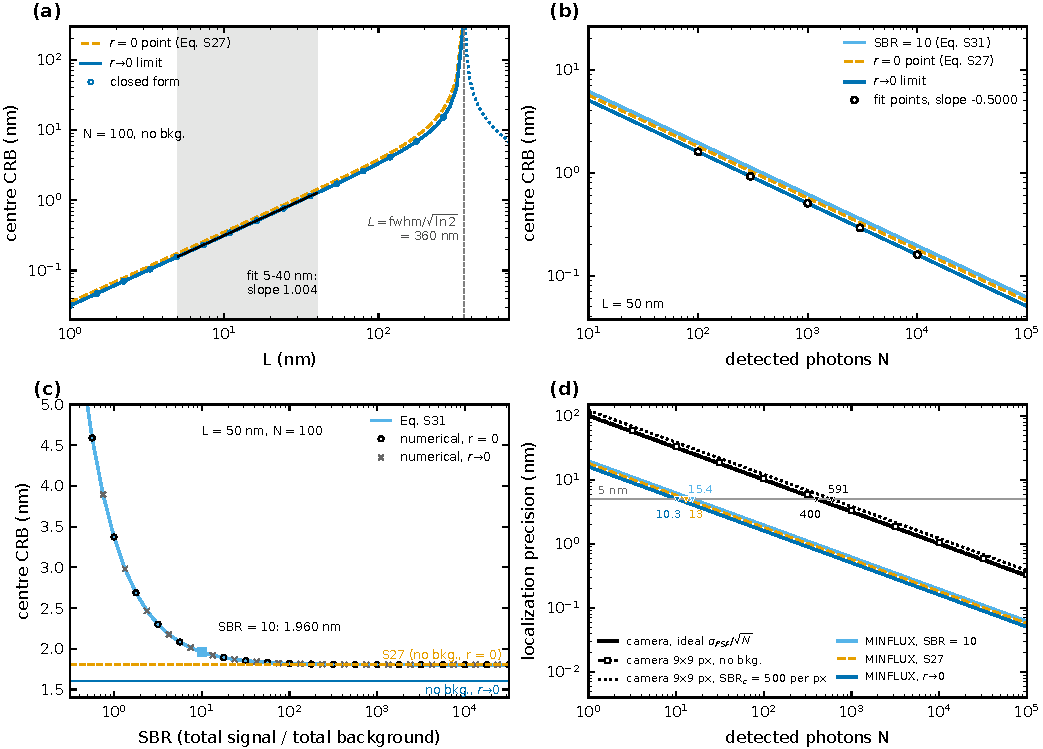
\includegraphics[width=\textwidth]{figures/fig4_scaling.pdf}
\caption{Scaling of the centre CRB and comparison with camera localization. (a)~CRB versus $L$
($N=100$, no background): $r\to0$ limit (numerical and closed form) and point value of
Eq.~\eqref{eq:s27}; the log--log slope fitted over $L=5$--$40$\,nm (shaded, $L\ll\fwhm$) is
\pnum{crb_exponent_L}\src{crb_exponent_L}. With a perfect zero the CRB increases monotonically
only for $L$ below the ring diameter
\pnum{eps0_crb_divergence_L_nm}\src{eps0_crb_divergence_L_nm}\,nm, diverges there and decreases
beyond (dotted). (b)~CRB versus $N$ for $L=50$\,nm: slope $-1/2$ for the limit, the point value
and Eq.~\eqref{eq:s31} with $\sbr=10$. (c)~CRB versus SBR ($L=50$\,nm, $N=100$): for finite SBR
the point value equals the limit (Eq.~\eqref{eq:s31}) and, as $\sbr\to\infty$, tends to the
point value of Eq.~\eqref{eq:s27}, not to the background-free limit. (d)~MINFLUX ($L=50$\,nm)
versus a camera ($\sigma_{\mathrm{PSF}}=100$\,nm): continuum limit $\sigma_{\mathrm{PSF}}/\sqrt N$
and a $9\times9$ window of $100$\,nm pixels, without background (dashed, nearly coincident with
the continuum line) and with $\sbr_c=500$ defined per pixel (total SBR \pnum{camera_sbr_perpixel_to_total}\src{camera_sbr_perpixel_to_total});
triangles mark the photons needed for $5$\,nm: $400$ for the ideal camera
(\pnum{camera_ideal_N400_nm}\src{camera_ideal_N400_nm}\,nm at $N=400$),
\pnum{camera_photons_for_5nm_perpixel_sbr500}\src{camera_photons_for_5nm_perpixel_sbr500} for
the pixelated camera with background, and for MINFLUX
\pnum{photons_for_5nm_L50_limit_nobg}\src{photons_for_5nm_L50_limit_nobg} with the $r\to0$
limit, \pnum{photons_for_5nm_L50_sbrinf}\src{photons_for_5nm_L50_sbrinf} with the point value
and \pnum{photons_for_5nm_L50_sbr10}\src{photons_for_5nm_L50_sbr10} with $\sbr=10$.}
\label{fig:scaling}
\end{figure*}
